\documentclass[conference]{IEEEtran}

\usepackage{amsmath}
\usepackage{blindtext}
\usepackage{graphicx}
\usepackage[utf8]{inputenc}
\usepackage[x11names, rgb, dvipsnames]{xcolor}
\usepackage{xfrac}

\usepackage{tikz}
\usetikzlibrary{snakes,arrows,shapes}

\bibliographystyle{plain}

\DeclareMathOperator{\orig}{orig}
\DeclareMathOperator{\dest}{dest}

\DeclareMathOperator{\calls}{calls}
\DeclareMathOperator{\etime}{time}
\DeclareMathOperator{\sms}{sms}
\DeclareMathOperator{\contacts}{contacts}

\DeclareMathOperator{\incalls}{incalls}
\DeclareMathOperator{\intime}{intime}
\DeclareMathOperator{\insms}{insms}
\DeclareMathOperator{\incontacts}{incontacts}

\DeclareMathOperator{\outcalls}{outcalls}
\DeclareMathOperator{\outtime}{outtime}
\DeclareMathOperator{\outsms}{outsms}
\DeclareMathOperator{\outcontacts}{outcontacts}

\DeclareMathOperator{\ego}{Ego}

\newcommand{\todo}[1]{\textbf{\color{red} TODO:\@ #1}}
\newcommand{\maybe}[1]{\footnote{\color{red} #1}}

\newcommand{\noimage}{%
  \setlength{\fboxsep}{-\fboxrule}
  \fbox{\phantom{\rule{\columnwidth}{100pt}}}
}
\newcommand{\includegraphicsmaybe}[1]{\IfFileExists{#1}{\includegraphics[width=\columnwidth]{#1}}{\noimage}}

\title{Comparison of Feature Extraction Methods and Predictors for Income Inference}

\author{%
\IEEEauthorblockN{%
	Martin Fixman\IEEEauthorrefmark{1},
	Carlos Sarraute\IEEEauthorrefmark{2},
	Many Others\IEEEauthorrefmark{2}
}
\IEEEauthorblockA{\IEEEauthorrefmark{1}Universidad de Buenos Aires, Argentina}
\IEEEauthorblockA{\IEEEauthorrefmark{2}Grandata Labs, Bartolomé Cruz 1818, Vicente López, Buenos Aires, Argentina}
\IEEEauthorblockA{martinfixman@gmail.com, charles@grandata.com}
}

\begin{document}
\maketitle

\begin{abstract}
Obtaining and processing demographical and sociological data have been some of the most important processes for understanding population-wide phenomena since at least 17th century~\cite{friendly2006}, and finding simple and intuitive ways of visualizing them has a big impact in our ways of understanding the data~\cite{minard1844,snow1855}. Common ways of obtaining useful qualitative data on socioeconomic stratification usually involved archival research or social surveys~\cite{bulmer1977}; however those methods can't present data that's at the same time exact, up to date, and that applies to a large population without having to rely on statistical methods.

Telecommunication operators (``telcos'') have access to a wealth of information about their users' communications and habits~\cite{huurdeman2003}, but the ability to store and process that data has taken large strides in the last few years thanks to new and more powerful computers and data mining techniques. The same can be said for sociological and economic information owned by banks and credit cards, and the relation between these two data sources.

Large scale data mining of data from the telecommunications industry is a relatively new area that's been so far mostly used for internal applications~\cite{han2002emerging}, but the gigantic wealth of real-time sociological data has been of interest for academic purposes related to sociology. This thesis builds on methods used by Óskardottir et.\ al.~\cite{oskardottir2016} and Singh et.\ al~\cite{singh2013predicting}, along with a large dataset of information for a certain telco and a large bank to find that the income distribution of the users follows closely (but not exactly) the income distribution of the whole population.

There's a strong homophily between the incomes of contacts in the telco, which along with the uneven distribution of wealth in the population is leveraged to create a methodology, grounded in Bayesian statistics, to infer socioeconomic level of a large subset of users in the network without banking information which is very accurate at $\AUC = 0.746$. The Bayesian method is later compared to several other methods based on supervised machine learning to prove that, even though it uses less input information, it's a better predictor of social features in this particular kind of network.

% In this work, we examine the socio-economic correlations present among users in a mobile phone network. First, we find that the distribution of income for a subset of users, for which we have income information given by a large bank, follows closely, but not exactly, the income distribution for the whole population. We also show the existence of a strong socio-economic homophily in the mobile phone network, where users linked in the network are more likely to have similar income. The main contribution of this work is that we leverage this homophily in order to propose a methodology, based on Bayesian statistics, to infer the socio-economic status for a large subset of users in the network (for which we have no banking information). With our proposed algorithm, we create an estimator for two categories (low and high income) which significantly outperforms both a simpler method based on a frequentist approach and several common \emph{Machine Learning} methods.

\end{abstract}

% !TEX root = tesis.tex

\chapter{Introduction}

% MOTIVATION
\section{Motivation of the Thesis}

In recent years, we have witnessed an exponential growth in the capacity to gather, store and manipulate massive amounts of data across a broad spectrum of disciplines: in astrophysics our capacity to gather and analyze massive datasets from astronomical observations has significantly transformed our capacity to model the dynamics of our cosmos; in sociology our capacity to track and study traits from individuals within a population of millions is allowing us to create social models at multiple scales, tracking individual and collective behavior both in space and time, with a granularity not even imagined twenty years ago.

In particular, mobile phone datasets provide a very rich view into the social interactions and the physical movements of large segments of a population. The voice calls and text messages exchanged between people, together with the call locations (recorded through cell tower usages), allow us to construct a rich social graph which can give us interesting insights on the users' social fabric, detailing not only particular social relationships and traits, but also regular patterns of behavior both in space and time, such as their daily and weekly mobility patterns~\cite{gonzalez2008understanding,ponieman2013human,sarraute2015city}.

Demographic factors play an important role in the constitution and preservation of social links. In particular concerning their age, individuals have a tendency to
establish links with others of similar age. This phenomenon is called age homophily~\cite{mcpherson2001birds}, and has been verified in mobile phone communications graph~\cite{blumenstock2010mobile,sarraute2014} as well as the Facebook graph~\cite{ugander2011anatomy}.


% PREVIOUS WORK ON THIS PROBLEM

Economic factors are also believed to have a determining role in both the social network's structure and dynamics. However, there are still very few large-scale quantitative analyses on the interplay between economic status of individuals and their social network. In~\cite{leo2015socioeconomic}, the authors analyze the correlations between mobile phone data and banking transaction information, revealing the existence of social stratification. They also show the presence of socioeconomic homophily among the networks participants using users' income, purchasing power and debt as indicators.
The authors of \cite{Luo2017inferring} studied the correlation between the position of a node in a mobile phone communications graph and its socio-economic status. They showed that the position and topological attributes in the graph can be used to generate inferences of the users' financial status.
In particular the study \cite{Luo2017inferring} shows the value of the Collective Influence~\cite{morone2015influence} as a topological attribute for the prediction of individual financial status.


% SUMMARY OF THE NEW APPROACH
\section{Summary of our Approach}

In this work, we leverage the socioeconomic homophily present in the cellular phone network to generate inferences of socioeconomic status in the communication graph. To this aim we will use the following data sources: (i) the Call Detail Records (CDRs) from the operator allow us to construct a social graph and to establish social affinities among users; (ii) banking reported income for a subset of their clients obtained from a large bank data source. We then construct an inferential algorithm that allows us to predict the socioeconomic status of users close to those for which we have banking information. To our knowledge, this is the first time both mobile phone and banking information has been integrated in this way to make inferences based on a social telecommunication graph.
Part of this work was published in~\cite{Fixman2016bayesian}.

The work done on this thesis is based the hypotheses that there is a significant level of homophily between a person's socioeconomic level and the one from its contacts (\cref{subsec:income_homophily}), and that using this correlation we can infer the first from the second (\cref{subsec:prediction_algorithm}).
At the same time, this thesis presents several ``conventional'' Machine Learning algorithms (\cref{sec:comparison}) along with an inference algorithm based in Bayesian Inference which works thanks to the correlation hypothesis (\cref{sec:inference_methodology}). This extra information should give this algorithm better results than the conventional ones.

Multiple strategies can be used to generate network features based on the CDRs. For instance, in \cite{oskarsdottir2016} the authors evaluate different collective inference methods applied to the churn prediction problem. Furthermore, the work \cite{oskarsdottir2017social} studies the impact of the social graph definition on the performance of the prediction methods. This motives the second part of the thesis, where we perform a comparative study of methods to generate network features for the nodes in the communication graph, and evaluate their impact on the inference of the income. We also compare the effectiveness of machine learning methods such as Logistic Regression and Random Forest on the different feature sets.

\todo{Add a summary of results}

\section{Organisation of the Thesis}

The remainder of the thesis is organized as follows.
In Chapter~\ref{chap:theoretical_intro} we provide an introduction to the theoretical ideas used in the thesis: the concept of homophily in social networks, \todo{complete}.

In Chapter~\ref{chap:related_work} we review related work on correlations in social-economic networks and on relation between socioeconomic status and mobile phone use. ETC \todo{complete}.

Chapter~\ref{sec:dataset} reviews the data sources used in this study. \todo{complete}.





% !TEX root = feature_extraction.tex

\section{Data Sources}
\label{sec:data_sources}

\subsection{Mobile Phone Data Source}
\label{subsec:telcoinformation}

The data used in this study consist of a set $P$ of \textit{Call Detail Records} (CDRs), composed of voice calls and another set $S$ containing text messages, from a telecommunication company (\textit{telco}) in a Latin American country for a period of 3 consecutive months.

Every CDR $p \in P$ contains the phone numbers of the caller (origin) and callee (destination) $\left< p_o, p_d \right>$, which are anonymized using a cryptographic hash function for privacy reasons; the starting time \( p_t \); and the call duration \( p_s \). The same datum, except call duration, can be found for each element $s \in S$.

Given that our collections $P$ and $S$ are coming from one mobile phone company, we are able to reconstruct all communication links between clients of this company, as well as communications between the clients and other users, but we have no information on communications where neither users are clients of the telco. Since we need all the information about the calls and SMS messages of the users in the graph, we work only with the clients of the mobile phone operator to generate inferences.

\subsection{Banking Information}

For this study we also had access to the set $B$ of account balances of over 10 million clients of a bank for a period of 6 consecutive months in the same country (with the same endpoint than the period of time %described in \cref{subsec:telcoinformation}). 
of the mobile phone datasource).
The data of each client $b \in B$ contains the phone number $b_p$ anonymized with the same cryptographic function as the datasets of \cref{subsec:telcoinformation}, along with the reported income of this person over 6 months $b_{s_1}, \ldots, b_{s_6}$. We average these 6 values to get $b_s$, an estimate of the users' monthly income.

Since the objective of this paper is to detect users with high income, we simplify the task by % not using or predicting the number directly. Instead, we
grouping the users into two equally-sized categories, one with \emph{Low Income} users and another for users with \emph{High Income}, which are simply defined as the high and low quantile of users, as shown in \cref{eq:lowhighincome},
where $m$ is the median of the income distribution.

\begin{equation}
\label{eq:lowhighincome}
\begin{gathered}
	\left| \left\{ b \in B \mid b_s \leq m \right\} \right| \approx \left| \left\{ b \in B \mid b_s > m \right\} \right| \\
	H_{b_p} = \begin{cases} \text{Low} & \text{if} \ b_s \leq m \\ \text{High} & \text{if} \ b_s > m \end{cases}
\end{gathered}
\end{equation}

\subsection{Bank-Telco Matching}

Since the phone numbers in each call or message made by the clients of the mobile phone operator is anonymized with the same hash function as the phone number registered in the bank dataset $B$, we can define several values for the intersection of the bank and telco datasets as the set of CDRs $P'$, and the income information in $H$. This approach is summarized in \cref{eq:banktelcomatching}.

\begin{equation}
\label{eq:banktelcomatching}
\begin{aligned}
	V_B &= \bigcup_{b \in B} b_p \\
	P' &= \left\{ p \in P \mid p_o \in V_B \lor p_d \in V_B \right\}
\end{aligned}
\end{equation}



\section{Basic Graph Features}
\label{sec:graphfeatures}

We represent the network as a directed graph $G = \left< V, E \right>$, where the nodes $V$ represent the users and the links $E$ represent the links between them.

This graph is created from the data presented in \cref{sec:data_sources}: $V$ is simply the union of all the origin and destination numbers on the intersection of either $P$ or $S$ and the set of numbers from the telco, and $E$ contains one element for every pair of nodes in either direction where the data is the accumulation of the number of calls, the total time of those calls, and the number of text messages.


A small subset of the nodes, $T \subseteq V$ contains the \emph{Ground Truth} of the data, which tells whether that user is part of the group of users with \emph{High Income} or the one with \emph{Low Income}. This data will be useful to train the predictors, test them, and also for generating some features as seen in \cref{subsec:categoricaluserdata}.

$E$ contains the accumulated data of the edges between nodes. Each element $e \in E$ contains the following information.

\begin{itemize}
	\item \textbf{Origin} of the calls and SMS, which is the incoming endpoint of this edge in the graph.
	\item \textbf{Destination} of the calls and SMS, which is the outgoing endpoint of this edge of the graph.
	\item \textbf{Calls}, the total number of calls from the origin to the destination.
	\item \textbf{Time}, the total time (in seconds) of all the calls from the origin to the destination.
	\item \textbf{SMS}, the total amount of messages from the origin to the destination.
\end{itemize}

There isn't a simple way to use the three quantifiable features (\emph{Calls}, \emph{Time}, and \emph{SMS}) directly, since they refer to information about the edges when there should be a prediction towards the nodes. However, as shown in \cref{sec:accumulatedfeatures}, this data, along with the information in $T$, can be accumulated for each user in different ways in order to create features for each user which are possible to use in the prediction of socioeconomic levels.


\section{Accumulated Graph Features}
\label{sec:accumulatedfeatures}

This section presents several ways of transforming data from the graph $G = \left< V, E \right>$ into individual features for each user $v \in V$.

The inferences are classified into named levels depending on the transformation done to $G$, and they are merged with levels containg less information as specified in Figure~\ref{fig:mlrelationships}. The total amount of columns in each featureset is presented in Table~\ref{tab:features}.

\begin{table}
\centering
\begin{tabular}{>{\bfseries}l r}
\toprule
Level & Features \\
\midrule
$\ego_0$ & \num{8}  \\
$\ego_1$ & \num{16} \\
$\ego_2$ & \num{24} \\
$\cat_0$ & \num{24} \\
$\cat_1$ & \num{48} \\
$\cat_2$ & \num{72} \\
\bottomrule
\end{tabular}
\caption{Amount of total features per level.}
\label{tab:features}
\end{table}

\begin{figure}
\centering
\resizebox{!}{.2\textheight}{%
	\framebox{%
		
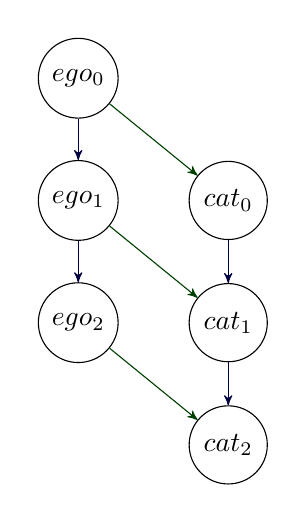
\begin{tikzpicture}[>=latex,line join=bevel,]
%%
\begin{scope}
  \pgfsetstrokecolor{black}
  \definecolor{strokecol}{rgb}{1.0,1.0,1.0};
  \pgfsetstrokecolor{strokecol}
  \definecolor{fillcol}{rgb}{1.0,1.0,1.0};
  \pgfsetfillcolor{fillcol}
  \filldraw (0.0bp,0.0bp) -- (0.0bp,168.0bp) -- (90.0bp,168.0bp) -- (90.0bp,0.0bp) -- cycle;
\end{scope}
\begin{scope}
  \pgfsetstrokecolor{black}
  \definecolor{strokecol}{rgb}{1.0,1.0,1.0};
  \pgfsetstrokecolor{strokecol}
  \definecolor{fillcol}{rgb}{1.0,1.0,1.0};
  \pgfsetfillcolor{fillcol}
  \filldraw (0.0bp,0.0bp) -- (0.0bp,168.0bp) -- (90.0bp,168.0bp) -- (90.0bp,0.0bp) -- cycle;
\end{scope}
\begin{scope}
  \pgfsetstrokecolor{black}
  \definecolor{strokecol}{rgb}{1.0,1.0,1.0};
  \pgfsetstrokecolor{strokecol}
  \definecolor{fillcol}{rgb}{1.0,1.0,1.0};
  \pgfsetfillcolor{fillcol}
  \filldraw (0.0bp,0.0bp) -- (0.0bp,168.0bp) -- (90.0bp,168.0bp) -- (90.0bp,0.0bp) -- cycle;
\end{scope}
\begin{scope}
  \pgfsetstrokecolor{black}
  \definecolor{strokecol}{rgb}{1.0,1.0,1.0};
  \pgfsetstrokecolor{strokecol}
  \definecolor{fillcol}{rgb}{1.0,1.0,1.0};
  \pgfsetfillcolor{fillcol}
  \filldraw (0.0bp,0.0bp) -- (0.0bp,168.0bp) -- (90.0bp,168.0bp) -- (90.0bp,0.0bp) -- cycle;
\end{scope}
  \node (d0p) at (72.0bp,106.0bp) [draw,circle] {$cat_0$};
  \node (d1p) at (72.0bp,62.0bp) [draw,circle] {$cat_1$};
  \node (d2p) at (72.0bp,18.0bp) [draw,circle] {$cat_2$};
  \coordinate (inv2) at (18.0bp,18.0bp);
  \coordinate (inv0) at (72.0bp,150.0bp);
  \node (0) at (18.0bp,150.0bp) [draw,circle] {$ego_0$};
  \node (1) at (18.0bp,106.0bp) [draw,circle] {$ego_1$};
  \node (2) at (18.0bp,62.0bp) [draw,circle] {$ego_2$};
  \definecolor{strokecolor}{rgb}{0.0,0.25,0.0};
  \draw [strokecolor,-stealth'] (2) ..controls (37.602bp,46.028bp) and (43.91bp,40.888bp)  .. (d2p);
  \definecolor{strokecolor}{rgb}{0.0,0.0,0.25};
  \draw [strokecolor,-stealth'] (d1p) ..controls (72.0bp,43.69bp) and (72.0bp,43.53bp)  .. (d2p);
  \definecolor{strokecolor}{rgb}{0.0,0.25,0.0};
  \draw [strokecolor,-stealth'] (1) ..controls (37.602bp,90.028bp) and (43.91bp,84.888bp)  .. (d1p);
  \definecolor{strokecolor}{rgb}{0.0,0.25,0.0};
  \draw [strokecolor,-stealth'] (0) ..controls (37.602bp,134.03bp) and (43.91bp,128.89bp)  .. (d0p);
  \definecolor{strokecolor}{rgb}{0.0,0.0,0.25};
  \draw [strokecolor,-stealth'] (d0p) ..controls (72.0bp,87.69bp) and (72.0bp,87.53bp)  .. (d1p);
  \definecolor{strokecolor}{rgb}{0.0,0.0,0.25};
  \draw [strokecolor,-stealth'] (0) ..controls (18.0bp,131.69bp) and (18.0bp,131.53bp)  .. (1);
  \definecolor{strokecolor}{rgb}{0.0,0.0,0.25};
  \draw [strokecolor,-stealth'] (1) ..controls (18.0bp,87.69bp) and (18.0bp,87.53bp)  .. (2);
%
\end{tikzpicture}


	}
}
\caption{Relationships between the \emph{Feature Extraction} methods of Section~\ref{sec:accumulatedfeatures}. \textcolor{Blue}{Blue} edges represent a raise in \emph{Ego Network} size, a process which is describe in Section~\ref{subsec:higherorderuserdata}, while \textcolor{ForestGreen}{green} edges represent adding label information, which is described in Section~\ref{subsec:categoricaluserdata}}
\label{fig:mlrelationships}
\end{figure}

\subsection{User Data --- Level $\ego_0$}
\label{subsec:user_data}

The first accumulated features consist of accumulating the three quantifiable features described in Section~\ref{sec:graphfeatures} for every node, separated on whether those features are incoming or outgoing.

Additionally, we add two features corresponding to the \emph{In-Degree} and \emph{Out-Degree} of each node. This can be seen as the sum of an imaginary feature on each link $e \in E$, \textbf{Contacts}, which is always exactly $1$ when the link exists.

These features are defined mathematically for each node $v \in V$ in Equation~\ref{eq:user_data}.

\begin{equation}
\begin{gathered}
\begin{aligned}
\incalls_v &= \sum_{\substack{e \in E \\ e_d = v}} \calls_e &
\outcalls_v &= \sum_{\substack{e \in E \\ e_o = v}} \calls_e \\
\intime_v &= \sum_{\substack{e \in E \\ e_d = v}} \etime_e &
\outtime_v &= \sum_{\substack{e \in E \\ e_o = v}} \etime_e \\
\insms_v &= \sum_{\substack{e \in E \\ e_d = v}} \sms_e &
\outsms_v &= \sum_{\substack{e \in E \\ e_o = v}} \sms_e \\
\end{aligned} \\
\begin{aligned}
\incontacts_v &= \left| \left\{ e \in E \mid e_d = v \right\} \right| \\
\outcontacts_v &= \left| \left\{ e \in E \mid e_o = v \right\} \right|
\end{aligned}
\end{gathered}
\label{eq:user_data}
\end{equation}

These accumulated patterns present interesting distributions which are similar in all telcos. These distributions are presented in Figure~\ref{fig:callsms}, Figure~\ref{fig:time}, and Figure~\ref{fig:contacts}.

\begin{figure}
\includegraphicsmaybe{figures/outcalls_dist.png}
\caption{Distribution of the amount of calls in the graph.}
\label{fig:callsms}
\end{figure}

\begin{figure}
\includegraphicsmaybe{figures/avg_time_hist.png}
\caption{Distribution of average call time.}
\label{fig:time}
\end{figure}

\begin{figure}
\includegraphicsmaybe{figures/outcontacts_dist.png}
\caption{Distribution of degree for all users.}
\label{fig:contacts}
\end{figure}

\subsection{Higher Order User Data --- Level $\ego_{n > 0}$}
\label{subsec:higherorderuserdata}

The features described in Section~\ref{subsec:user_data} correspond to the information about calls and SMS from a user $v \in V$ towards all of its neighbours. However, there's no reason why this information can't be extended to nodes at a higher distance from $v$.

The \emph{Ego Network} of the node $v$ is defined as the graph consisting of $v$ and its neighbors. A simple way to get more features about that node is to accumulate the call and SMS information about the edges which are \textbf{not} part of the \emph{Ego Network}, but one endpoint on the border of this.

Additionally, if we define the distance between two nodes using the intuitive definition which is presented on Equation~\ref{eq:distance}, we can define the \emph{User Data of Order $n$}, for any natural number $n$, as the accumulation of call and SMS information where one endpoint is on the border of the \emph{Ego Network of Order $n$}, and the other one isn't. The \emph{Ego Network of Order $n$} of a certain node $v$ is the subgraph composed of the node $v$, plus all the nodes which are at most at distance $n$ of $v$.

\begin{equation}
d \left( a, b \right) =
\begin{cases}
	0 & \text{if } a = b \\
	1 + \min_{v \in \neigh \left(b \right)} d \left( a, v \right) & \text{otherwise}
\end{cases}
\label{eq:distance}
\end{equation}

\begin{table*}[t]
\begin{tabular*}{\textwidth}{>{\bfseries}l >{\bfseries}l >{\bfseries}l @{\extracolsep{\fill}}>{\hspace{2em}}r r r r r r >{\hspace{2em}}r >{\hspace{-1em}}r}
\toprule
Dataset & Model & Level & Accuracy & Precision & Recall & AUC & F\textsubscript{1}-score & F\textsubscript{4}-score & Fit Time & Predict Time \\
\midrule

\multirow{15}{*}{\centering Inner Graph}

& \multicolumn{2}{>{\bfseries}l}{Random Selection}
& 0.499 & 0.499 & 0.500 & 0.499 & 0.500 & 0.500 & \NA{} & \SI{0.005}{\second} \\

& \multicolumn{2}{>{\bfseries}l}{Majority Voting}
& 0.681 & 0.640 & 0.826 & 0.681 & 0.721 & 0.712 & \NA{} & \SI{0.059}{\second} \\

& \multicolumn{2}{>{\bfseries}l}{Bayesian Algorithm}

& 0.693 & 0.665 & 0.792 & 0.746 & 0.723 & 0.783 & \NA{} & \SI{33.155}{\second} \\
\cmidrule{2-11}

& \multirow{5}{*}{LR} &
   $\ego_0$ & 0.536 & 0.531 & 0.625 & 0.536 & 0.574 & 0.619 & \SI{0.145}{\second}   & \SI{0.002}{\second} \\
&& $\ego_1$ & 0.535 & 0.525 & 0.730 & 0.535 & 0.611 & 0.714 & \SI{0.141}{\second}   & \SI{0.011}{\second} \\
&& $\ego_2$ & 0.568 & 0.578 & 0.525 & 0.569 & 0.550 & 0.528 & \SI{0.119}{\second}   & \SI{0.003}{\second} \\
&& $\cat_0$ & 0.686 & 0.655 & 0.785 & 0.686 & 0.714 & 0.776 & \SI{0.167}{\second}   & \SI{0.005}{\second} \\
&& $\cat_1$ & 0.693 & 0.665 & 0.780 & 0.693 & 0.718 & 0.772 & \SI{1.588}{\second}   & \SI{0.011}{\second} \\
&& $\cat_2$ & 0.693 & 0.670 & 0.764 & 0.692 & 0.714 & 0.758 & \SI{0.956}{\second}   & \SI{0.009}{\second} \\
\cmidrule{2-11}

& \multirow{5}{*}{RF} &
   $\ego_0$ & 0.548 & 0.548 & 0.550 & 0.548 & 0.549 & 0.550 & \SI{5.986}{\second}   & \SI{0.588}{\second} \\
&& $\ego_1$ & 0.582 & 0.583 & 0.577 & 0.582 & 0.580 & 0.577 & \SI{56.548}{\second}  & \SI{0.483}{\second} \\
&& $\ego_2$ & 0.576 & 0.577 & 0.580 & 0.576 & 0.579 & 0.580 & \SI{50.197}{\second}  & \SI{0.253}{\second} \\
&& $\cat_0$ & 0.671 & 0.665 & 0.690 & 0.671 & 0.677 & 0.688 & \SI{6.346}{\second}   & \SI{0.539}{\second} \\
&& $\cat_1$ & \textbf{0.714} & \textbf{0.713} & \textbf{0.716} & \textbf{0.714} & \textbf{0.714} & \textbf{0.716} & \SI{96.005}{\second}  & \SI{0.460}{\second} \\
&& $\cat_2$ & 0.709 & 0.710 & 0.711 & 0.709 & 0.711 & 0.711 & \SI{81.528}{\second}  & \SI{0.242}{\second} \\
\midrule

\multirow{14}{*}{\centering Outer Graph}

& \multicolumn{2}{>{\bfseries}l}{Random Selection}
&       0.499 & 0.499 & 0.500 & 0.499 & 0.500 & 0.500 & \NA{} & \SI{0.005}{\second} \\

& \multicolumn{2}{>{\bfseries}l}{Majority Voting}
&       0.565 & 0.747 & 0.197 & 0.565 & 0.312 & 0.206 & \NA{} & \SI{0.204}{\second} \\
\cmidrule{2-11}

& \multirow{5}{*}{LR} &
   $\ego_0$ & 0.534 & 0.586 & 0.234 & 0.534 & 0.335 & 0.243 & \SI{0.937}{\second}   & \SI{0.016}{\second} \\
&& $\ego_1$ & 0.547 & 0.617 & 0.250 & 0.547 & 0.356 & 0.260 & \SI{1.347}{\second}   & \SI{0.035}{\second} \\
&& $\ego_2$ & 0.563 & 0.586 & 0.430 & 0.563 & 0.496 & 0.437 & \SI{1.055}{\second}   & \SI{0.023}{\second} \\
&& $\cat_0$ & 0.565 & 0.746 & 0.198 & 0.565 & 0.313 & 0.207 & \SI{1.871}{\second}   & \SI{0.041}{\second} \\
&& $\cat_1$ & 0.577 & 0.727 & 0.247 & 0.577 & 0.368 & 0.257 & \SI{9.816}{\second}   & \SI{0.077}{\second} \\
&& $\cat_2$ & 0.589 & 0.636 & 0.415 & 0.589 & 0.503 & 0.424 & \SI{9.456}{\second}   & \SI{0.065}{\second} \\
\cmidrule{2-11}

& \multirow{5}{*}{RF} &
   $\ego_0$ & 0.543 & 0.544 & 0.529 & 0.543 & 0.536 & 0.530 & \SI{25.789}{\second}  & \SI{4.878}{\second} \\
&& $\ego_1$ & 0.578 & 0.585 & 0.537 & 0.578 & 0.560 & 0.540 & \SI{102.961}{\second} & \SI{5.608}{\second} \\
&& $\ego_2$ & 0.583 & 0.590 & 0.541 & 0.583 & 0.564 & 0.543 & \SI{70.447}{\second}  & \SI{3.148}{\second} \\
&& $\cat_0$ & 0.568 & 0.573 & 0.536 & 0.568 & 0.554 & 0.538 & \SI{32.981}{\second}  & \SI{5.371}{\second} \\
&& $\cat_1$ & 0.613 & 0.634 & 0.533 & 0.613 & 0.579 & 0.538 & \SI{44.911}{\second}  & \SI{6.002}{\second} \\
&& $\cat_2$ & 0.614 & 0.635 & 0.534 & 0.614 & 0.580 & 0.539 & \SI{50.589}{\second}  & \SI{3.484}{\second} \\
\bottomrule
\end{tabular*}
\caption{Resulting metrics of different methods used in Section~\ref{sec:results} tested on both the \emph{Inner Graph}, which contains only nodes which have at least one neighbour with socioeconomic information, and the \emph{Outer Graph}, which includes all nodes. \textbf{Bolded} items represent the highest value for each metric which is being presented in this paper.}
\label{tab:comparison}
\end{table*}


This definition can be seen intuitively in Figure~\ref{fig:higherorderuserdata}. For reference purposes, we assign the level $\ego_0$ to the information of the regular \emph{User Data} from Section~\ref{subsec:user_data}, while the user data from the \emph{Ego Network of Order $n$} is assigned $ego_n$ for some $n > 0$\footnotemark{}.

\footnotetext{Note that the first definition isn't necessary; we could just say that the \emph{User Data of Order 0} contains information about the edges adjacent to \emph{Ego Network of Order 0}, which are the edges user in the regular User Data. This is the reason why the \emph{User Data} has level $\ego_0$.}

\begin{figure}
\centering
\framebox[\columnwidth]{%
	
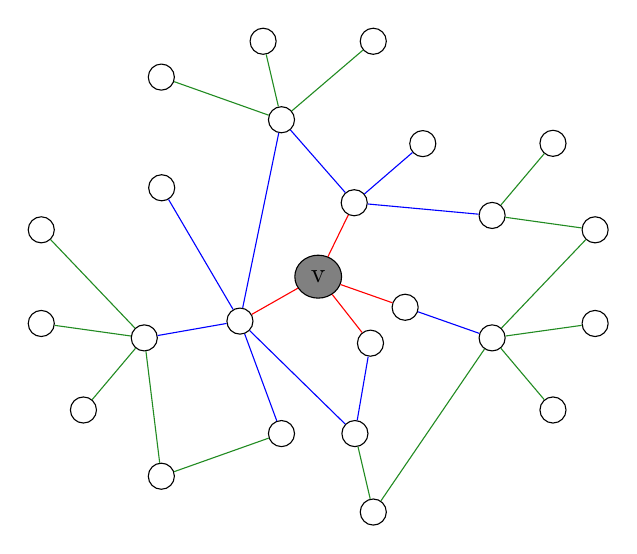
\begin{tikzpicture}[>=latex,line join=bevel,]
%%
\node (b4) at (58.264bp,80.697bp) [draw,ellipse] {};
  \node (b5) at (107.65bp,46.247bp) [draw,ellipse] {};
  \node (b6) at (134.09bp,46.247bp) [draw,ellipse] {};
  \node (b7) at (183.48bp,80.697bp) [draw,ellipse] {};
  \node (b0) at (183.48bp,124.78bp) [draw,ellipse] {};
  \node (b1) at (158.52bp,150.63bp) [draw,ellipse] {};
  \node (b2) at (107.65bp,159.23bp) [draw,ellipse] {};
  \node (b3) at (64.526bp,134.74bp) [draw,ellipse] {};
  \node (c11) at (64.398bp,30.901bp) [draw,ellipse] {};
  \node (c10) at (36.354bp,54.739bp) [draw,ellipse] {};
  \node (a1) at (92.698bp,86.739bp) [draw,ellipse] {};
  \node (a0) at (133.84bp,129.35bp) [draw,ellipse] {};
  \node (c9) at (21.176bp,85.884bp) [draw,ellipse] {};
  \node (a2) at (139.69bp,78.794bp) [draw,ellipse] {};
  \node (c3) at (140.7bp,18.0bp) [draw,ellipse] {};
  \node (c2) at (220.56bp,85.884bp) [draw,ellipse] {};
  \node (c1) at (205.39bp,54.739bp) [draw,ellipse] {};
  \node (c0) at (220.56bp,119.6bp) [draw,ellipse] {};
  \node (c7) at (205.39bp,150.74bp) [draw,ellipse] {};
  \node (c6) at (64.398bp,174.58bp) [draw,ellipse] {};
  \node (c5) at (101.04bp,187.48bp) [draw,ellipse] {};
  \node (c4) at (140.7bp,187.48bp) [draw,ellipse] {};
  \node (a3) at (152.17bp,91.719bp) [draw,ellipse] {};
  \node (c8) at (21.176bp,119.6bp) [draw,ellipse] {};
  \node (v) at (120.87bp,102.74bp) [draw,fill=gray,ellipse] {v};
  \draw [red,] (v) ..controls (135.03bp,84.728bp) and (135.11bp,84.621bp)  .. (a2);
  \draw [ForestGreen,] (b6) ..controls (138.26bp,28.429bp) and (138.28bp,28.341bp)  .. (c3);
  \draw [blue,] (a1) ..controls (80.328bp,107.82bp) and (76.815bp,113.8bp)  .. (b3);
  \draw [ForestGreen,] (b7) ..controls (166.4bp,55.662bp) and (157.67bp,42.867bp)  .. (c3);
  \draw [blue,] (a0) ..controls (121.21bp,143.76bp) and (120.45bp,144.63bp)  .. (b2);
  \draw [ForestGreen,] (b2) ..controls (87.533bp,166.37bp) and (84.387bp,167.49bp)  .. (c6);
  \draw [ForestGreen,] (b4) ..controls (41.841bp,97.922bp) and (37.585bp,102.39bp)  .. (c8);
  \draw [red,] (v) ..controls (142.36bp,95.175bp) and (142.44bp,95.145bp)  .. (a3);
  \draw [ForestGreen,] (b7) ..controls (199.9bp,97.922bp) and (204.16bp,102.39bp)  .. (c0);
  \draw [blue,] (a0) ..controls (147.71bp,141.31bp) and (147.8bp,141.39bp)  .. (b1);
  \draw [ForestGreen,] (b0) ..controls (195.28bp,138.77bp) and (195.36bp,138.87bp)  .. (c7);
  \draw [ForestGreen,] (b4) ..controls (61.028bp,58.262bp) and (61.616bp,53.483bp)  .. (c11);
  \draw [ForestGreen,] (b2) ..controls (103.48bp,177.05bp) and (103.46bp,177.14bp)  .. (c5);
  \draw [blue,] (a1) ..controls (74.544bp,83.554bp) and (74.414bp,83.531bp)  .. (b4);
  \draw [red,] (v) ..controls (130.88bp,123.29bp) and (130.94bp,123.4bp)  .. (a0);
  \draw [ForestGreen,] (b7) ..controls (195.28bp,66.71bp) and (195.36bp,66.613bp)  .. (c1);
  \draw [blue,] (a0) ..controls (156.36bp,127.28bp) and (160.96bp,126.85bp)  .. (b0);
  \draw [ForestGreen,] (b4) ..controls (46.458bp,66.71bp) and (46.377bp,66.613bp)  .. (c10);
  \draw [blue,] (a3) ..controls (169.4bp,85.652bp) and (169.52bp,85.612bp)  .. (b7);
  \draw [ForestGreen,] (b5) ..controls (87.533bp,39.109bp) and (84.387bp,37.993bp)  .. (c11);
  \draw [ForestGreen,] (b2) ..controls (123.17bp,172.5bp) and (124.91bp,173.98bp)  .. (c4);
  \draw [blue,] (a1) ..controls (99.753bp,67.634bp) and (100.57bp,65.415bp)  .. (b5);
  \draw [blue,] (a2) ..controls (136.61bp,60.878bp) and (136.59bp,60.759bp)  .. (b6);
  \draw [red,] (v) ..controls (100.85bp,91.371bp) and (100.71bp,91.289bp)  .. (a1);
  \draw [blue,] (a1) ..controls (110.72bp,69.108bp) and (116.32bp,63.636bp)  .. (b6);
  \draw [blue,] (a1) ..controls (98.712bp,115.9bp) and (101.69bp,130.32bp)  .. (b2);
  \draw [ForestGreen,] (b7) ..controls (201.88bp,83.271bp) and (202.17bp,83.312bp)  .. (c2);
  \draw [ForestGreen,] (b4) ..controls (39.861bp,83.271bp) and (39.566bp,83.312bp)  .. (c9);
  \draw [ForestGreen,] (b0) ..controls (201.88bp,122.21bp) and (202.17bp,122.17bp)  .. (c0);
%
\end{tikzpicture}


}
\caption{Example of the edges present in the calculation of the \emph{Higher Order User Data} for a certain node $v$. \textcolor{red}{Red} edges represent edges whose features are accumulated in the \emph{User Data of Order 0}, \textcolor{blue}{blue} edges represent those of \emph{Order 1}, and \textcolor{ForestGreen}{green} those of \emph{Order 2}.}
\label{fig:higherorderuserdata}
\end{figure}

\subsection{Categorical User Data --- Level $\cat_n$}
\label{subsec:categoricaluserdata}

Another approach to building features for the test is to combine the information contained in $E$, the list of edges, with the one in the ground truth $T \subseteq V$, which says whether a certain node represents a person of \emph{High Income} or a person of \emph{Low Income}.

A simple way to do that is to do an approach similar to the \emph{User Data} presented in Section~\ref{subsec:user_data}, but further discriminating each feature which corresponds to a node $v \in V$ and an edge $e \in E$ when $t \in T$ is the other endpoint of $e$ on whether $t$ corresponds to a person with high or low income. The resulting new features are of the form represented by the set in Equation~\ref{eq:matcatuserdata}.

\begin{equation}
\begin{Bmatrix} in \\ out \end{Bmatrix}
\times
\begin{Bmatrix} calls \\ time \\ sms \\ contacts \end{Bmatrix}
\times
\begin{Bmatrix} low \\ high \end{Bmatrix}
\label{eq:matcatuserdata}
\end{equation}

It's important to keep in mind that not all edges of $G$ will be accumulated to these features. Indeed, the majority of users in the testing set $T$ don't have any neighbour that's also in $T$, and thus every feature in this category ends up being $0$.

For completeness sake the set of nodes $F \subseteq T$ is defined as the nodes in the \emph{Inner Graph} (in contrast to the \emph{Outer Graph}, that contains all nodes in $T$), where $F$ only contains nodes which have at least one neighbour with socioeconomic information. In Section~\ref{sec:results} we'll include information about both graphs, and naturally the results on the \emph{Inner Graph} will be better than the ones in the \emph{Outer Graph}, since it contains more information.

Creating these features naïvely will occur in overfitting, since the features are generated by data that's also used for training the supervised learning models. To solve this, the set $T$ is partitioned into two disjoint sets, $G$ and $H$, where $G$ contains roughly 0.75 of the nodes in $T$ is used to calculate the features, while $H$ contains the other 0.25 and is used to train the models.

It's possible to use the method presented in Section~\ref{subsec:higherorderuserdata} generate an \emph{Ego Network of level $n$} of a certain node $v$, and accumulate the adjacent nodes to that network by socioeconomic level before accumulating their data. We refer to the level of these features as $\cat_n$.


\bibliography{bibliography/sna}{}

\end{document}
